\begin{wrapfigure}{r}{0.4\linewidth}
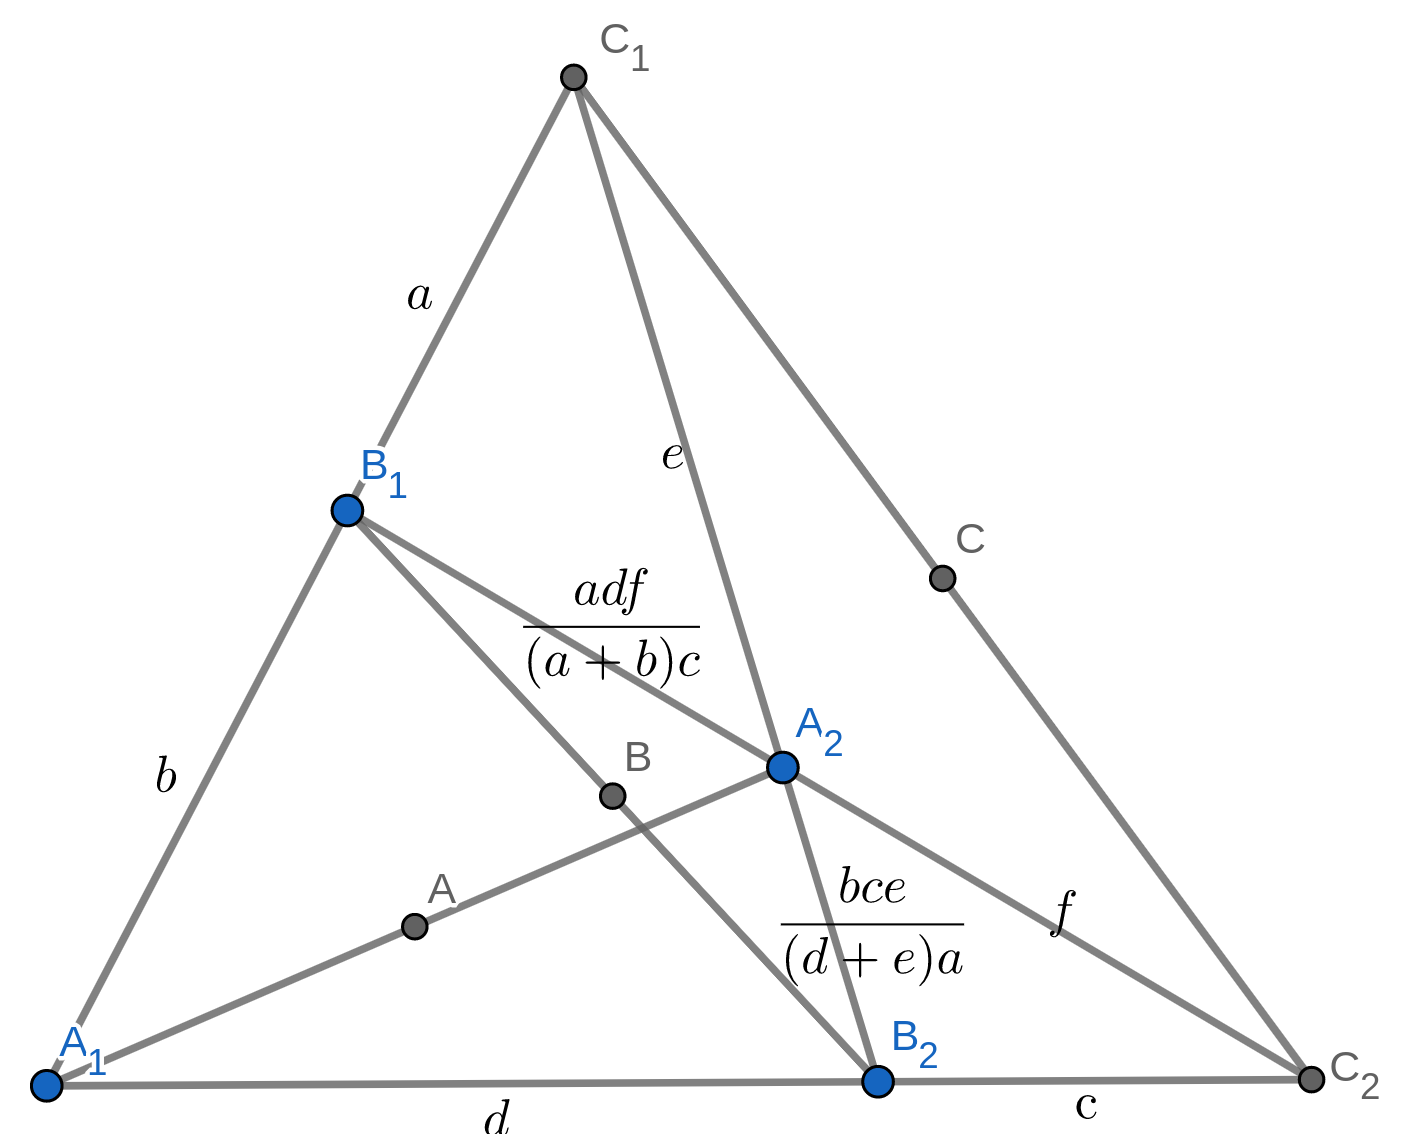
\includegraphics[width=\linewidth]{tasks/Гаусс жив.png}
\end{wrapfigure}

Пускай отрезки имеют длины такие же какие указаны на рисунке (длины отрезков $B_1A_2$ и $B_2A_2$ вычислены из других с помощью теоремы Менелая). Тогда поставим массу $-\frac{2bc}{a(c+d)} =(-\frac{bc}{ad}) +  \frac{bc(c-d)}{ad(c+d)}$ в $C_1$,
$-\frac{2bc}{a(c+d)} = -\frac{2bc+ac+ad}{a(c+d)} + 1$ в $C_2$,
$\frac{2c(a+b)}{ad} = \frac{c(a+b)}{ad} + \frac{c(a+b)}{ad}$ в  $B_1$
и $\frac{2c(a+b)}{ad} = \frac{ad+2bc+ac}{ad} + \frac{c-d}{d}$ в $B_2$. Тогда, т. к. в вершинах $C_1$ и  $C_2$ находятся одинаковые массы, заменим их на их центр масс в точке $C$. Аналогично заменим $B_1$ и  $B_2$ на $B$. Таким образом центр масс системы из этих четырех точек лежит на прямой $BC$, найдем его. 

Для этого найдем центр масс части точки $C_1$ с массой $(-\frac{bc}{ad})$ и части точки $B_1$ с массой $\frac{c(a+b)}{ad}$. Это точка $A_1$, т. к. $A_1B_1 \cdot \frac{c(a+b)}{ad} + A_1C_1 \cdot (-\frac{bc}{ad})= \frac{abc+b^2c}{ad} -\frac{abc + b^2c}{ad} = 0$. Также для части точки $C_2$ с массой $(-\frac{2bc+ac+ad}{a(c+d)})$ и части точки $B_2$ с массой $\frac{ad+2bc+ac}{ad}$ центр масс также $A_1$, т. к. $A_1B_2 \cdot \frac{ad+2bc+ac}{ad} + A_1C_2 \cdot (-\frac{2bc+ac+ad}{a(c+d)})= \frac{ad+2bc+ac}{a} -\frac{2bc+ac+ad}{a} = 0$. Таким образом в точке $A_1$ скопилась сумма этих масс, а именно масса $-\frac{bc}{ad}-\frac{2bc+ac+ad}{a(c+d)}+\frac{c(a+b)}{ad}+\frac{ad+2bc+ac}{ad}=\frac{2c(a+b)}{ad}+1-\frac{2bc+ac+ad}{a(c+d)}=\frac{2c(ac+ad+bc)}{ad(c+d)}$. Для оставшихся частей масс в точках также найдем их центр. Для части точки $C_1$ с массой $\frac{bc(c-d)}{ad(c+d)}$ и части точки $B_2$ с массой $\frac{c-d}{d}$ это точка $A_2$, т. к. $C_1A_2 \cdot \frac{bc(c-d)}{ad(c+d)} = \frac{bce(c-d)}{ad(c+d)} = A_2B_2 \cdot \frac{c-d}{d}$. Осталось найти центр масс части точки $B_1$ с массой $\frac{c(a+b)}{ad}$ и части точки $C_2$ с массой $1$, это точка $A_2$, т. к. $B_1A_2 \cdot \frac{c(a+b)}{ad} = f = A_2C_2 \cdot 1$. Таким образом в точке $A_1$ скопилась сумма этих масс, а именно масса $\frac{bc(c-d)}{ad(c+d)} + \frac{c-d}{d} + \frac{c(a+b)}{ad} + 1 = \frac{c}{d}(\frac{b(c-d)}{a(c+d)} + 1 + \frac{(a+b)}{a}) = (\frac{c}{d})\frac{bc-bd+ac+ad+ac+bc+ad+bd}{a(c+d)} = \frac{2c(ac+ad+bc)}{ad(c+d)}$. 

\begin{wrapfigure}{r}{0.05\linewidth}
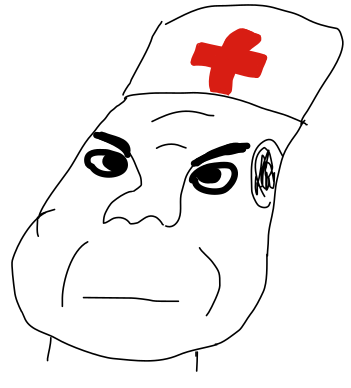
\includegraphics[width=\linewidth]{tasks/SXKj17wSmm.png}
\end{wrapfigure}

Мы свели нашу систему точек к двум точкам $A_1$ и $A_2$ с равными массами, значит центр масс системы находится в середине отрезка $A_1A_2$ в точке $A$. 
Ранее мы доказали, что центр масс лежит на прямой $BC$, тогда $A$ лежит на прямой $BC$ ч. т. д.

%\frac{bc^2-bcd+ac^2-ad^2 + ac^2 +acd+bc^2+bcd + acd + ad^2}{ad(c+d)} = \frac{ac^2 + ac^2 +acd+ acd}{ad(c+d)}=\frac{2c(c +d)}{ad(c+d)}=\frac{2c}{ad}$

